\documentclass{AnantDocumentation}
\usepackage{tikz}
\usetikzlibrary{shapes.geometric, arrows.meta, positioning, fit, backgrounds}
\backgroundsetup{
	contents=""
}


\title{ECE F434 Project Report: Audio Watermarking}
\author{Meghadri Ghosh - 2023A3PS0314P \\ Pramit Pal - 2023AAPS0765P \\ Pranav Chandra N. V. - 2023AAPS0013P}

\begin{document}
\begin{center}
	{\Large ECE F434 Project Report: Audio Watermarking \par}
	\vspace{0.3cm}
	{\normalsize Meghadri Ghosh - 2023A3PS0314P \\ Pramit Pal - 2023AAPS0765P \\ Pranav Chandra N. V. - 2023AAPS0013P \par}
\end{center}

\section{Approach}
The reference paper by Yamni et al. combines three transforms to encrypt and embed an image as a binary watermark into the low frequency components of an audio signal. We replicate their method and analyze its performance under various attacks. (\href{https://github.com/Meghadri25/dsp-project}{\textbf{Github Repo}})

We embed a binary watermark using chaotic encryption, wavelet decomposition and Tchebichef moment modulation. We begin with the chaotic encryption, MLNCML, where we use a map defined by $\epsilon = 0.4, \mu = 3.99$ to generate a chaotic bit-plane $H_b$. 
The watermark $W$ is then encrypted using exor operation: 
\begin{equation}
W' = W \oplus H_b .
\end{equation}
The audio is simultaneously divided into $L_{\text{seg}} = \left\lceil \frac{N M}{L_1} \right\rceil = 256$ segments, and each undergoes a 3-level Haar DWT:
\begin{equation}
\text{DWT}^3(\text{segment}) \rightarrow (A_3, D_3, D_2, D_1),
\end{equation}
with embedding performed in the low-frequency block \( A_3 \). This block is split into \( L_1 = 4 \) sub-blocks, and each is transformed using DTMT with $K = \min(64, L_2/2)$ Tchebichef orders:
\begin{equation}
M = T\,\text{pa3}, \qquad T \in \mathbb{R}^{K \times L_2}.
\end{equation}
Moments are separated as even and odd components, and a bit \( b \) is embedded by adjusting their norms. With
\begin{equation}
\bar{\sigma} = \frac{\|M_1\| + \|M_2\|}{2}, \qquad \delta = 0.05,
\end{equation}
the modified norms are
\begin{equation}
(\sigma_1',\sigma_2') =
\begin{cases}
(\bar{\sigma}+\delta,\ \bar{\sigma}-\delta), & b=1,\\
(\bar{\sigma}-\delta,\ \bar{\sigma}+\delta), & b=0.
\end{cases}
\end{equation}
Reconstruction uses the inverse DTMT,
\begin{equation}
\text{pa3}' = T^{T} M',
\end{equation}
followed by inverse DWT to obtain the watermarked segment.
During extraction, the bit is detected by comparing norms:
\begin{equation}
\hat{b} = \mathbf{1}\!\left(\|M_1\| > \|M_2\|\right),
\end{equation}
and the final watermark is recovered via
\begin{equation}
\hat{W} = \hat{W}' \oplus H_b .
\end{equation}

Figure \ref{fig:flowchart} in the appendix illustrates the complete enxryption and decryption pipeline.

\section{Testing and Results}
\subsection{Testing}
The paper proposes a few different kinds of attacks that they tested their watermarking system against. We used a few of these tests(1-4) as well as proposed some new ones(5-7) in order to extend the robustness analysis of the watermarking system.
\begin{enumerate}
	\item \textbf{Cropping by 20\%: } We remove 20\% of random audio samples from the watermarked audio to simulate random data loss.
	\item \textbf{Gaussian Noise of $20dB$: } We add white Gaussian noise to the watermarked audio such that the resulting SNR is 20 dB.
	\item \textbf{High-Pass Filter at 100Hz}
	\item \textbf{Low-Pass Filter at 4kHz}
	\item \textbf{MP3 compression at 32, 64 and 128 kbps: } To simulate lossy compression, we encode and decode the watermarked audio using MP3 compression.
	\item \textbf{Random Time Scaling by $\pm 20\%$: } We randomly speed up or slow down the watermarked audio by up to 20\%.
	\item \textbf{Re-recording: } We simulate re-recording by playing the watermarked audio through speakers and capturing it with a microphone. 
\end{enumerate}

Table \ref{tab:results} summarizes the results of these attacks on the audio and watermark. The SNR and BER 
\begin{table}[h]
\centering
\begin{tabular}{@{}lcccccc@{}}
\toprule
\textbf{Attack} & \textbf{SNR (dB)} & \textbf{SI-SDR} & \textbf{BER} & \textbf{NC} &  \textbf{LMSE} & \textbf{SSIM}\\
\midrule
No Attack &7.734&6.933&0.000&1.000&0.000 & 1.000\\
20\% Crop &4.749	&2.977	&0.104	&0.792	&1.808	&0.263\\ 
Gaussian 20dB & 7.525	& 6.683	& 0.004	& 0.993	& 0.043	&0.989 \\
HPF 100Hz & 1.742	&-2.868	& 0.322	& 0.356	& 3.749	& 0.159 \\
LPF 4kHz & 6.808 & 5.794 & 0.0199	& 0.960	& 0.380 & 0.598 \\ 
MP3 32kbps & 6.669	& 5.643	& 0.180	& 0.640	& 2.811	& 0.181 \\
MP3 64kbps & 7.379	& 6.538	& 0.075	& 0.850	& 1.317	& 0.357 \\
MP3 128kbps & 7.662	& 6.909	& 0.001	& 0.998	& 0.015	& 0.973 \\
Time Scale $\pm 20\%$ & -1.457	& -38.571	& 0.499	& 0.002	& 5.313	& 0.002\\
Re-recording & 1.842	& -0.274	& 0.483	& 0.035	& 5.262	& 0.008 \\
\bottomrule
\end{tabular}
\caption{Audio (SNR and SI-DBR) and Watermark (BER, NC, LMSE, SSIM) quality metrics under various attacks}
\label{tab:results}
\end{table}

\subsection{Results}
In order to effectively demonstrate the watermarking, the original and encrypted watermarks are shown in Figure \ref{fig:watermarks}.
\begin{figure}[h!]
	\centering
	\begin{subfigure}{0.4\textwidth}
		\centering
		\includegraphics[width=0.5\textwidth]{../watermark.png}
		\label{fig:original_watermark}
	\end{subfigure}
	\hfill
	\begin{subfigure}{0.4\textwidth}
		\centering
		\includegraphics[width=0.5\textwidth]{../results/extract_results/extracted_watermark.png}
		\label{fig:encrypted_watermark}
	\end{subfigure}
	\caption{Original watermark (left) and extracted watermark with no attack (right)}
	\label{fig:watermarks}
\end{figure}

You would note that the structure of the extracted image is very similar, with even fine details like the numbers on the dial being preserved.

Now, the attacked images are shown in figure \ref{fig:attacked_watermarks}.
\begin{figure}[h!]
    \centering
    % Row 1
    \begin{subfigure}{0.18\textwidth}
        \centering
        \includegraphics[width=\linewidth]{../results/extract_results/extracted_watermark.png}
		\caption{}
		\label{fig:encrypted and extracted watermark}
    \end{subfigure}
    \begin{subfigure}{0.18\textwidth}
        \centering
        \includegraphics[width=\linewidth]{../results/attack_results/CROP_20pct/extracted_watermark.png}
		\caption{}
		\label{fig:cropped watermark}
    \end{subfigure}
    \begin{subfigure}{0.18\textwidth}
        \centering
        \includegraphics[width=\linewidth]{../results/attack_results/GAUSS_noise_20dB/extracted_watermark.png}
		\caption{}
		\label{fig:gaussian noise watermark}
    \end{subfigure}
    \begin{subfigure}{0.18\textwidth}
        \centering
        \includegraphics[width=\linewidth]{../results/attack_results/HPF_100Hz/extracted_watermark.png}
		\caption{}
		\label{fig:high pass filter watermark}
    \end{subfigure}
    \begin{subfigure}{0.18\textwidth}
        \centering
        \includegraphics[width=\linewidth]{../results/attack_results/LPF_4000Hz/extracted_watermark.png}
		\caption{}
		\label{fig:low pass filter watermark}
    \end{subfigure}

    \vspace{0.3cm}

    % Row 2
    \begin{subfigure}{0.18\textwidth}
        \centering
        \includegraphics[width=\linewidth]{../results/attack_results/MP3_32kbps/extracted_watermark.png}
		\caption{}
		\label{fig:mp3 32kbps watermark}
    \end{subfigure}
    \begin{subfigure}{0.18\textwidth}
        \centering
		\includegraphics[width=\linewidth]{../results/attack_results/MP3_64kbps/extracted_watermark.png}
		\caption{}
		\label{fig:mp3 64kbps watermark}
    \end{subfigure}
    \begin{subfigure}{0.18\textwidth}
        \centering
		\includegraphics[width=\linewidth]{../results/attack_results/MP3_128kbps/extracted_watermark.png}
		\caption{}
		\label{fig:mp3 128kbps watermark}
    \end{subfigure}
    \begin{subfigure}{0.18\textwidth}
        \centering
        \includegraphics[width=\linewidth]{../results/attack_results/Random_time_scaling/extracted_watermark.png}
		\caption{}
		\label{fig:time scaled watermark}
    \end{subfigure}
    \begin{subfigure}{0.18\textwidth}
        \centering
        \includegraphics[width=\linewidth]{../results/attack_results/Re_recording/extracted_watermark.png}
		\caption{}
		\label{fig:re-recorded watermark}
    \end{subfigure}
	\caption{(a) No attack extraction (b) 20\% Crop (c) Gaussian Noise 20dB (d) HPF 100Hz (e) LPF 4kHz (f) MP3 32kbps (g) MP3 64kbps (h) MP3 128kbps (i) Random Time Scaling $\pm$10\% (j) Re-recording}
	\label{fig:attacked_watermarks}
\end{figure}

From the results, we see that this watermarking method is very effective against nearly all attacks, save for the HPF, re-recording and time scaling.
However, an important note is that the audio quality is significantly degraded in these two cases, as can be seen from the very low SNR and SI-SDR values in Table \ref{tab:results}.
This means that the low performance of the watermarking method is not the primary issue, as pirates or other adversaries would be unlikely to use such low-quality audio.
\newpage

\section*{Appendix: System Architecture}

Figure \ref{fig:flowchart} shows how the three transforms work together. The watermark flows through encryption, gets split across audio segments, and embeds into frequency-domain moments. Extraction reverses the process.

\begin{figure}[h]
\centering
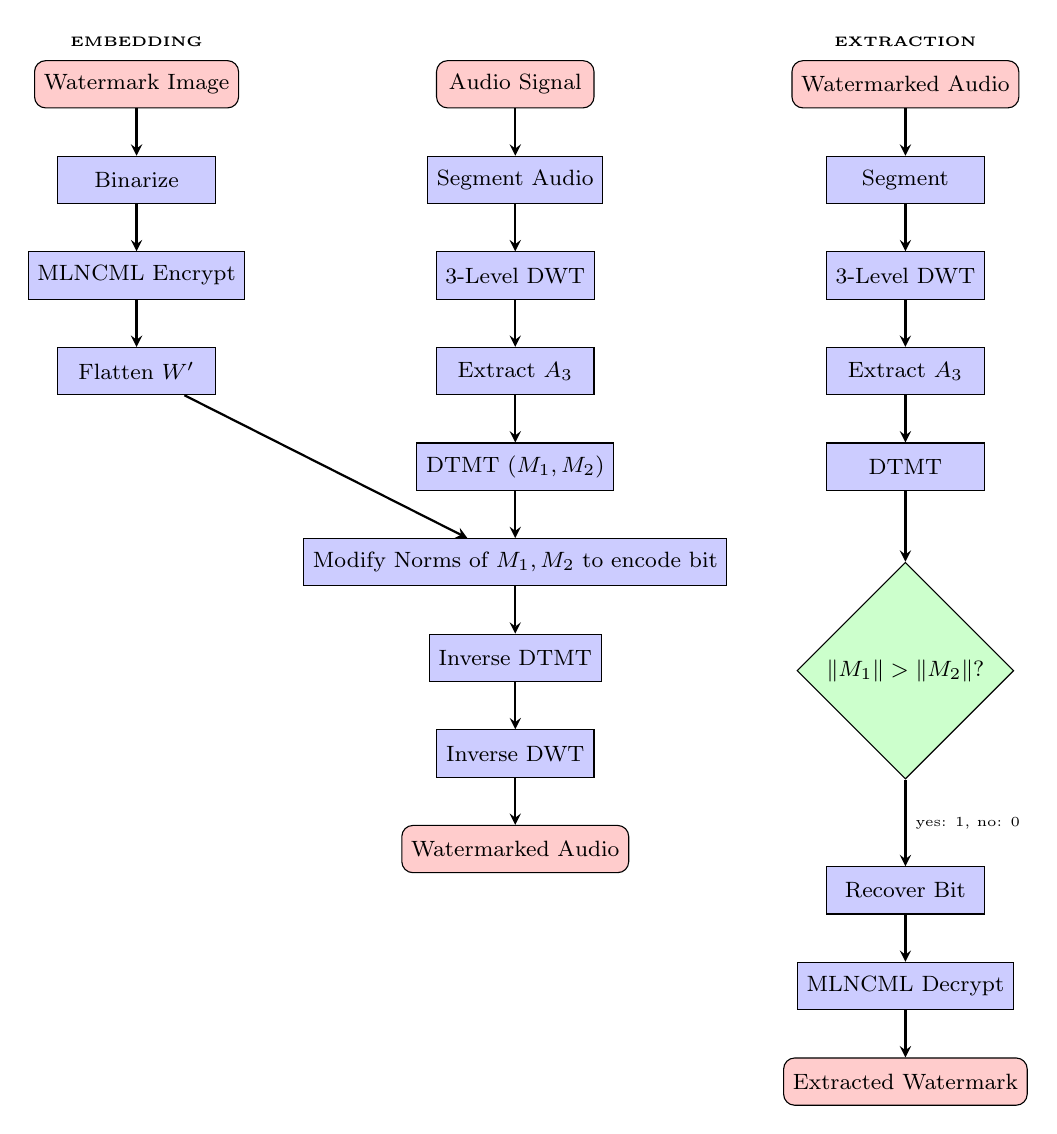
\begin{tikzpicture}[scale=1, every node/.style={transform shape},
    node distance=0.6cm and 1cm,
    startstop/.style={rectangle, rounded corners, minimum width=2cm, minimum height=0.6cm, text centered, draw=black, fill=red!20, font=\footnotesize},
    process/.style={rectangle, minimum width=2cm, minimum height=0.6cm, text centered, draw=black, fill=blue!20, font=\footnotesize},
    decision/.style={diamond, minimum width=1.5cm, minimum height=0.6cm, text centered, draw=black, fill=green!20, font=\footnotesize},
    arrow/.style={thick,->,>=stealth}
    ]
    
    % Embedding path
    \node (img) [startstop] {Watermark Image};
    \node (binarize) [process, below=of img] {Binarize};
    \node (mlncml) [process, below=of binarize] {MLNCML Encrypt};
    \node (flatten) [process, below=of mlncml] {Flatten $W'$};
    
    \node (audio) [startstop, right=2.5cm of img] {Audio Signal};
    \node (segment) [process, below=of audio] {Segment Audio};
    \node (dwt) [process, below=of segment] {3-Level DWT};
    \node (extract) [process, below=of dwt] {Extract $A_3$};
    \node (dtmt) [process, below=of extract] {DTMT ($M_1, M_2$)};
	\node (modify) [process, below=of dtmt] {Modify Norms of $M_1, M_2$ to encode bit};
    \node (idtmt) [process, below=of modify] {Inverse DTMT};
    \node (idwt) [process, below=of idtmt] {Inverse DWT};
    \node (watermarked) [startstop, below=of idwt] {Watermarked Audio};
    
    % Extraction path
    \node (wm_audio) [startstop, right=2.5cm of audio] {Watermarked Audio};
    \node (seg2) [process, below=of wm_audio] {Segment};
    \node (dwt2) [process, below=of seg2] {3-Level DWT};
    \node (a3_2) [process, below=of dwt2] {Extract $A_3$};
    \node (dtmt2) [process, below=of a3_2] {DTMT};
    \node (compare) [decision, below=of dtmt2, yshift=-0.3cm] {$\|M_1\| > \|M_2\|$?};
    \node (bit) [process, below=of compare, yshift=-0.5cm] {Recover Bit};
    \node (decrypt) [process, below=of bit] {MLNCML Decrypt};
    \node (extracted) [startstop, below=of decrypt] {Extracted Watermark};
    
    % Arrows - Embedding
    \draw [arrow] (img) -- (binarize);
    \draw [arrow] (binarize) -- (mlncml);
    \draw [arrow] (mlncml) -- (flatten);
    \draw [arrow] (audio) -- (segment);
    \draw [arrow] (segment) -- (dwt);
    \draw [arrow] (dwt) -- (extract);
    \draw [arrow] (extract) -- (dtmt);
    \draw [arrow] (flatten) -- (modify);
    \draw [arrow] (dtmt) -- (modify);
    \draw [arrow] (modify) -- (idtmt);
    \draw [arrow] (idtmt) -- (idwt);
    \draw [arrow] (idwt) -- (watermarked);
    
    % Arrows - Extraction
    \draw [arrow] (wm_audio) -- (seg2);
    \draw [arrow] (seg2) -- (dwt2);
    \draw [arrow] (dwt2) -- (a3_2);
    \draw [arrow] (a3_2) -- (dtmt2);
    \draw [arrow] (dtmt2) -- (compare);
    \draw [arrow] (compare) -- node[right, font=\tiny] {yes: 1, no: 0} (bit);
    \draw [arrow] (bit) -- (decrypt);
    \draw [arrow] (decrypt) -- (extracted);
    
    % Labels
    \node[above=0.05cm of img, font=\tiny\bfseries] {EMBEDDING};
    \node[above=0.05cm of wm_audio, font=\tiny\bfseries] {EXTRACTION};
    
\end{tikzpicture}
\caption{Watermarking system flowchart showing embedding (left/center) and extraction (right) pipelines}
\label{fig:flowchart}
\end{figure}

\end{document}

